\documentclass[twoside]{book}

% Packages required by doxygen
\usepackage{fixltx2e}
\usepackage{calc}
\usepackage{doxygen}
\usepackage[export]{adjustbox} % also loads graphicx
\usepackage{graphicx}
\usepackage[utf8]{inputenc}
\usepackage{makeidx}
\usepackage{multicol}
\usepackage{multirow}
\PassOptionsToPackage{warn}{textcomp}
\usepackage{textcomp}
\usepackage[nointegrals]{wasysym}
\usepackage[table]{xcolor}

% Font selection
\usepackage[T1]{fontenc}
\usepackage[scaled=.90]{helvet}
\usepackage{courier}
\usepackage{amssymb}
\usepackage{sectsty}
\renewcommand{\familydefault}{\sfdefault}
\allsectionsfont{%
  \fontseries{bc}\selectfont%
  \color{darkgray}%
}
\renewcommand{\DoxyLabelFont}{%
  \fontseries{bc}\selectfont%
  \color{darkgray}%
}
\newcommand{\+}{\discretionary{\mbox{\scriptsize$\hookleftarrow$}}{}{}}

% Page & text layout
\usepackage{geometry}
\geometry{%
  a4paper,%
  top=2.5cm,%
  bottom=2.5cm,%
  left=2.5cm,%
  right=2.5cm%
}
\tolerance=750
\hfuzz=15pt
\hbadness=750
\setlength{\emergencystretch}{15pt}
\setlength{\parindent}{0cm}
\setlength{\parskip}{3ex plus 2ex minus 2ex}
\makeatletter
\renewcommand{\paragraph}{%
  \@startsection{paragraph}{4}{0ex}{-1.0ex}{1.0ex}{%
    \normalfont\normalsize\bfseries\SS@parafont%
  }%
}
\renewcommand{\subparagraph}{%
  \@startsection{subparagraph}{5}{0ex}{-1.0ex}{1.0ex}{%
    \normalfont\normalsize\bfseries\SS@subparafont%
  }%
}
\makeatother

% Headers & footers
\usepackage{fancyhdr}
\pagestyle{fancyplain}
\fancyhead[LE]{\fancyplain{}{\bfseries\thepage}}
\fancyhead[CE]{\fancyplain{}{}}
\fancyhead[RE]{\fancyplain{}{\bfseries\leftmark}}
\fancyhead[LO]{\fancyplain{}{\bfseries\rightmark}}
\fancyhead[CO]{\fancyplain{}{}}
\fancyhead[RO]{\fancyplain{}{\bfseries\thepage}}
\fancyfoot[LE]{\fancyplain{}{}}
\fancyfoot[CE]{\fancyplain{}{}}
\fancyfoot[RE]{\fancyplain{}{\bfseries\scriptsize Generated by Doxygen }}
\fancyfoot[LO]{\fancyplain{}{\bfseries\scriptsize Generated by Doxygen }}
\fancyfoot[CO]{\fancyplain{}{}}
\fancyfoot[RO]{\fancyplain{}{}}
\renewcommand{\footrulewidth}{0.4pt}
\renewcommand{\chaptermark}[1]{%
  \markboth{#1}{}%
}
\renewcommand{\sectionmark}[1]{%
  \markright{\thesection\ #1}%
}

% Indices & bibliography
\usepackage{natbib}
\usepackage[titles]{tocloft}
\setcounter{tocdepth}{3}
\setcounter{secnumdepth}{5}
\makeindex

% Hyperlinks (required, but should be loaded last)
\usepackage{ifpdf}
\ifpdf
  \usepackage[pdftex,pagebackref=true]{hyperref}
\else
  \usepackage[ps2pdf,pagebackref=true]{hyperref}
\fi
\hypersetup{%
  colorlinks=true,%
  linkcolor=blue,%
  citecolor=blue,%
  unicode%
}

% Custom commands
\newcommand{\clearemptydoublepage}{%
  \newpage{\pagestyle{empty}\cleardoublepage}%
}

\usepackage{caption}
\captionsetup{labelsep=space,justification=centering,font={bf},singlelinecheck=off,skip=4pt,position=top}

%===== C O N T E N T S =====

\begin{document}

% Titlepage & ToC
\hypersetup{pageanchor=false,
             bookmarksnumbered=true,
             pdfencoding=unicode
            }
\pagenumbering{alph}
\begin{titlepage}
\vspace*{7cm}
\begin{center}%
{\Large My Project }\\
\vspace*{1cm}
{\large Generated by Doxygen 1.8.14}\\
\end{center}
\end{titlepage}
\clearemptydoublepage
\pagenumbering{roman}
\tableofcontents
\clearemptydoublepage
\pagenumbering{arabic}
\hypersetup{pageanchor=true}

%--- Begin generated contents ---
\chapter{album}
\label{md__r_e_a_d_m_e}
\Hypertarget{md__r_e_a_d_m_e}
\input{md__r_e_a_d_m_e}
\chapter{Hierarchical Index}
\section{Class Hierarchy}
This inheritance list is sorted roughly, but not completely, alphabetically\+:\begin{DoxyCompactList}
\item Test\+Case\begin{DoxyCompactList}
\item \contentsline{section}{Email\+Test}{\pageref{class_email_test}}{}
\end{DoxyCompactList}
\end{DoxyCompactList}

\chapter{Class Index}
\section{Class List}
Here are the classes, structs, unions and interfaces with brief descriptions\+:\begin{DoxyCompactList}
\item\contentsline{section}{\mbox{\hyperlink{class_email_test}{Email\+Test}} }{\pageref{class_email_test}}{}
\end{DoxyCompactList}

\chapter{File Index}
\section{File List}
Here is a list of all documented files with brief descriptions\+:\begin{DoxyCompactList}
\item\contentsline{section}{\mbox{\hyperlink{bd_8php}{bd.\+php}} \\*Файл для подключения к базе данных }{\pageref{bd_8php}}{}
\end{DoxyCompactList}

\chapter{Class Documentation}
\hypertarget{class_email_test}{}\section{Email\+Test Class Reference}
\label{class_email_test}\index{Email\+Test@{Email\+Test}}
Inheritance diagram for Email\+Test\+:\begin{figure}[H]
\begin{center}
\leavevmode
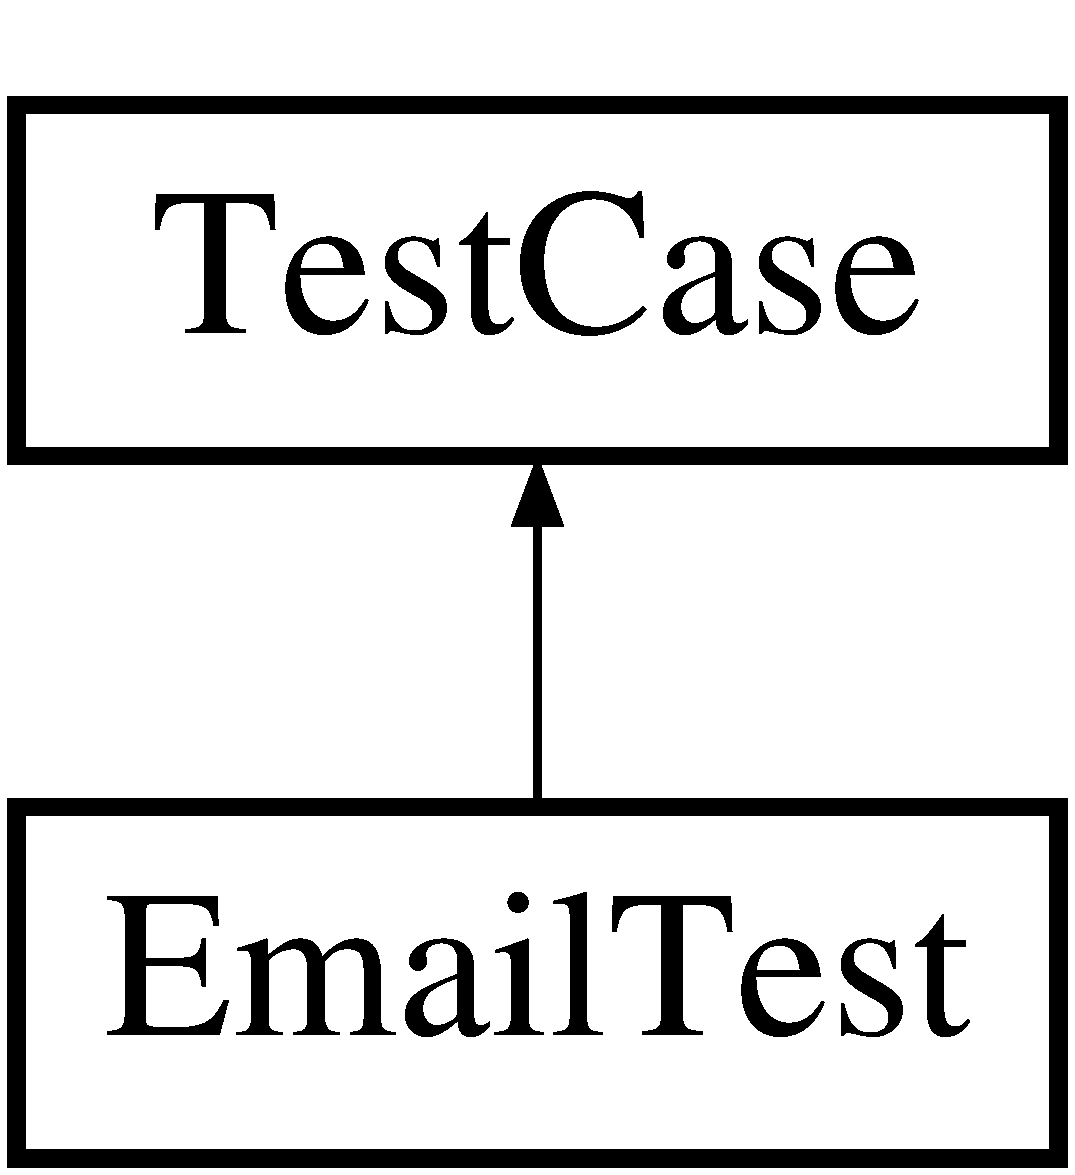
\includegraphics[height=2.000000cm]{class_email_test}
\end{center}
\end{figure}
\subsection*{Public Member Functions}
\begin{DoxyCompactItemize}
\item 
\mbox{\Hypertarget{class_email_test_a591d95d74a56bc17b0a4d132f845de66}\label{class_email_test_a591d95d74a56bc17b0a4d132f845de66}} 
{\bfseries test\+Power} ()
\end{DoxyCompactItemize}


The documentation for this class was generated from the following file\+:\begin{DoxyCompactItemize}
\item 
test.\+php\end{DoxyCompactItemize}

\chapter{File Documentation}
\hypertarget{bd_8php}{}\section{bd.\+php File Reference}
\label{bd_8php}\index{bd.\+php@{bd.\+php}}


Файл для подключения к базе данных  


\subsection*{Functions}
\begin{DoxyCompactItemize}
\item 
if(\$bd-\/$>$connect\+\_\+error) \mbox{\hyperlink{bd_8php_ab58fa0da68711c0ff0f09e5fecd02c21}{add\+File\+To\+Bd}} (\$name, \$orig, \$miniature, \$date, \$bd, \$model, \$lat, \$long)
\begin{DoxyCompactList}\small\item\em добавляет в базу данных информацию о фаойле \end{DoxyCompactList}\end{DoxyCompactItemize}
\subsection*{Variables}
\begin{DoxyCompactItemize}
\item 
\mbox{\Hypertarget{bd_8php_ad79b54e31bd1050001133c4d70f850fe}\label{bd_8php_ad79b54e31bd1050001133c4d70f850fe}} 
{\bfseries \$servername} = \char`\"{}localhost\char`\"{}
\item 
\mbox{\Hypertarget{bd_8php_a0eb82aa5f81cf845de4b36cd653c42cf}\label{bd_8php_a0eb82aa5f81cf845de4b36cd653c42cf}} 
{\bfseries \$username} = \char`\"{}User\char`\"{}
\item 
\mbox{\Hypertarget{bd_8php_a607686ef9f99ea7c42f4f3dd3dbb2b0d}\label{bd_8php_a607686ef9f99ea7c42f4f3dd3dbb2b0d}} 
{\bfseries \$password} = \char`\"{}123456789\char`\"{}
\item 
\mbox{\Hypertarget{bd_8php_ac5111a571fffa2499732833bb7f0d8c1}\label{bd_8php_ac5111a571fffa2499732833bb7f0d8c1}} 
{\bfseries \$dbname} = \char`\"{}album\char`\"{}
\item 
\mbox{\Hypertarget{bd_8php_acc3591d1c0945e5b934207901d1e06c0}\label{bd_8php_acc3591d1c0945e5b934207901d1e06c0}} 
{\bfseries \$bd} = new mysqli(\$servername, \$username, \$password,\$dbname)
\end{DoxyCompactItemize}


\subsection{Detailed Description}
Файл для подключения к базе данных 

Данный файл создает подключение к базе данных 

\subsection{Function Documentation}
\mbox{\Hypertarget{bd_8php_ab58fa0da68711c0ff0f09e5fecd02c21}\label{bd_8php_ab58fa0da68711c0ff0f09e5fecd02c21}} 
\index{bd.\+php@{bd.\+php}!add\+File\+To\+Bd@{add\+File\+To\+Bd}}
\index{add\+File\+To\+Bd@{add\+File\+To\+Bd}!bd.\+php@{bd.\+php}}
\subsubsection{\texorpdfstring{add\+File\+To\+Bd()}{addFileToBd()}}
{\footnotesize\ttfamily if ( \$bd-\/$>$connect\+\_\+error) add\+File\+To\+Bd (\begin{DoxyParamCaption}\item[{}]{\$name,  }\item[{}]{\$orig,  }\item[{}]{\$miniature,  }\item[{}]{\$date,  }\item[{}]{\$bd,  }\item[{}]{\$model,  }\item[{}]{\$lat,  }\item[{}]{\$long }\end{DoxyParamCaption})}



добавляет в базу данных информацию о фаойле 


\begin{DoxyParams}[1]{Parameters}
\mbox{\tt in}  & {\em name} & Имя добавляемого файла \\
\hline
\mbox{\tt in}  & {\em orig,miniature} & Ссылки на оригинальный файл и миниатюру \\
\hline
\mbox{\tt in}  & {\em date} & дата сьемки \\
\hline
\mbox{\tt in}  & {\em bd} & пременная подключения к бд \\
\hline
\mbox{\tt in}  & {\em model} & модель устройства \\
\hline
\mbox{\tt in}  & {\em lat,long} & широта и долгота места сьемки \\
\hline
\end{DoxyParams}
\begin{DoxyReturn}{Returns}
true в слечае успеха 
\end{DoxyReturn}

%--- End generated contents ---

% Index
\backmatter
\newpage
\phantomsection
\clearemptydoublepage
\addcontentsline{toc}{chapter}{Index}
\printindex

\end{document}
